
\documentclass[french]{beamer}

\usetheme{metropolis}
\usepackage{appendixnumberbeamer}
%\usepackage[scale=2]{ccicons}
%\usepackage{minted}
%\usepackage{booktabs}
%\usepackage[scale=2]{ccicons}

\usepackage{pgfplots}
\usepgfplotslibrary{dateplot}

\usepackage{xspace}
\newcommand{\themename}{\textbf{\textsc{metropolis}}\xspace}
\usepackage{pdfpages}
\usepackage{tikz}
\usepackage{tabularx}
% Package used for highlighting
\usepackage{soul}
% Package used for multirow tables
\usepackage{multirow}
\usepackage{graphicx}
\usepackage{textpos}
\usepackage{booktabs}
\usepackage{lipsum}% http://ctan.org/pkg/lipsum
\usepackage[normalem]{ulem}
\usepackage{transparent}

%INCOMPATIBLE AVEC FOOTNOTE
%\usepackage{setspace}% http://ctan.org/pkg/setspace
\usepackage{xcolor,colortbl}
\definecolor{nla}{HTML}{E6B71F}
\definecolor{sla}{HTML}{3EA4B9}
\newcommand{\nla}{\cellcolor{nla}}  %{0.9}
\newcommand{\sla}{\cellcolor{sla}}  %{0.9}
%\usepackage[scale=2]{ccicons}
%COLORS
\definecolor{olive}{rgb}{0.3, 0.4, .1}
%\definecolor{white}{HTML}{FFFFF}
\definecolor{fore}{RGB}{249,242,215}
\definecolor{back}{RGB}{51,51,51}
\definecolor{title}{RGB}{255,0,90}
\definecolor{dgreen}{rgb}{0.,0.6,0.}
\definecolor{gold}{rgb}{1.,0.84,0.}
\definecolor{JungleGreen}{cmyk}{0.99,0,0.52,0}
\definecolor{BlueGreen}{cmyk}{0.85,0,0.33,0}
\definecolor{RawSienna}{cmyk}{0,0.72,1,0.45}
\definecolor{Magenta}{cmyk}{0,1,0,0}
\definecolor{mygreen}{HTML}{033E37}
\definecolor{myred}{HTML}{E50707}
\definecolor{mylightgreen}{HTML}{00A339}
%\usefonttheme{structuresmallcapsserif} 

%\usefonttheme{smallcapsserif} 
\usefonttheme{serif} 
%\setsansfont[BoldFont={Source Sans Pro Semibold},           Numbers={OldStyle}]{Source Sans Pro}

%\metroset{titleformat=allsmallcaps}
%\usefonttheme{serif} % default family is serif
\setbeamercolor{frametitle}{bg=mygreen}
\setbeamercolor{example text}{fg=mylightgreen}
\setbeamercolor{alerted text}{fg=myred}
\usepgfplotslibrary{dateplot}
%Prevents arrow on x axis
\pgfplotsset{ every non boxed x axis/.append style={x axis line style=-}, every non boxed y axis/.append style={y axis line style=-}}
\newcommand{\tool}[1]{\texttt{#1}\xspace}
\newcommand{\cat}[1]{\textsc{#1}\xspace}
\newcommand{\variante}[1]{\textsc{#1}\xspace}
\renewcommand*{\thefootnote}{\alph{footnote}}

% Prevent section slide 
%\newcommand{\metropolis@disablesectionpage}{\AtBeginSection
%}

%%% CUSTOMIZING METROPOLIS
\metroset{sectionpage=none}
\metroset{numbering=none}
\metroset{block=transparent}
\newcommand\Wider[2][3em]{%
  \makebox[\linewidth][c]{%
    \begin{minipage}{\dimexpr\textwidth+#1\relax}
      \raggedright#2
    \end{minipage}%
  }%
}
\usepackage[utf8]{inputenc}
\usepackage[T1]{fontenc}
\usepackage[frenchb]{babel}

\setbeamerfont{frametitle}{shape=\scshape}
%\usepackage{setspace}

\title{\scshape Construction d'un corpus annoté en parties du discours
  \newline par myriadisation (\textit{crowdsourcing}) pour le traitement automatique d'une langue peu dotée : \newline l'alsacien}
 
%\subtitle{Analysis of the Participation on a Crowdsourcing Annotation Platform}
%\date{\today}
\author{Alice Millour, Kar\"en Fort}
\institute{Recherches linguistiques et corpus}
%\usecolortheme{rose}
%\setbeamercolor{structure}{fg=beamer@blendedblue} 
\begin{document}
\begin{frame}

    
  \tikz [remember picture,overlay]
  \node [shift={(+6.5cm,+1cm)}]  at (current page.south west)
  %or: (current page.center)
        {\includegraphics[width=1.5cm]{figures/logo-sorbonne-trans.png}};
        \titlepage
  \end{frame}


\begin{frame}{Introduction}
  \center
  %textbf{\large Crowdsourcing annotated data for \\ \vspace{0.2cm} less-resourced languages}
  %% \begin{itemize}
  %% \item ... to crowdsource linguistic annotations (POS tags so far)
  %% \item ... easy to adapt and easy to maintain.
  %% \end{itemize}  	
\end{frame}


\metroset{numbering=fraction}
\begin{frame}{Table of contents}
  \setbeamertemplate{section in toc}[sections numbered]
  \tableofcontents[hideallsubsections]
\end{frame}
\section{Quelques caractéristiques de l'alsacien}
\metroset{block=transparent}
%\metroset{exampleblock=transparent}
\begin{frame}{Plan}
  \setbeamertemplate{section in toc}[sections numbered]
  \tableofcontents[currentsection,hideothersubsections]
\end{frame}

% present our general results and show how our observations of the participation so far helps indicates us the future gamified features we want to develelop.
\subsection{L'alsacien}
\begin{frame}[fragile]{L'alsacien}
  %\begin{frame}[fragile]
  %\frametitle{\textsc{Typography}} 
  \Wider[4em]{\begin{columns}
      \begin{column}{0.5\textwidth}
        \begin{tikzpicture}
          \node (img0) {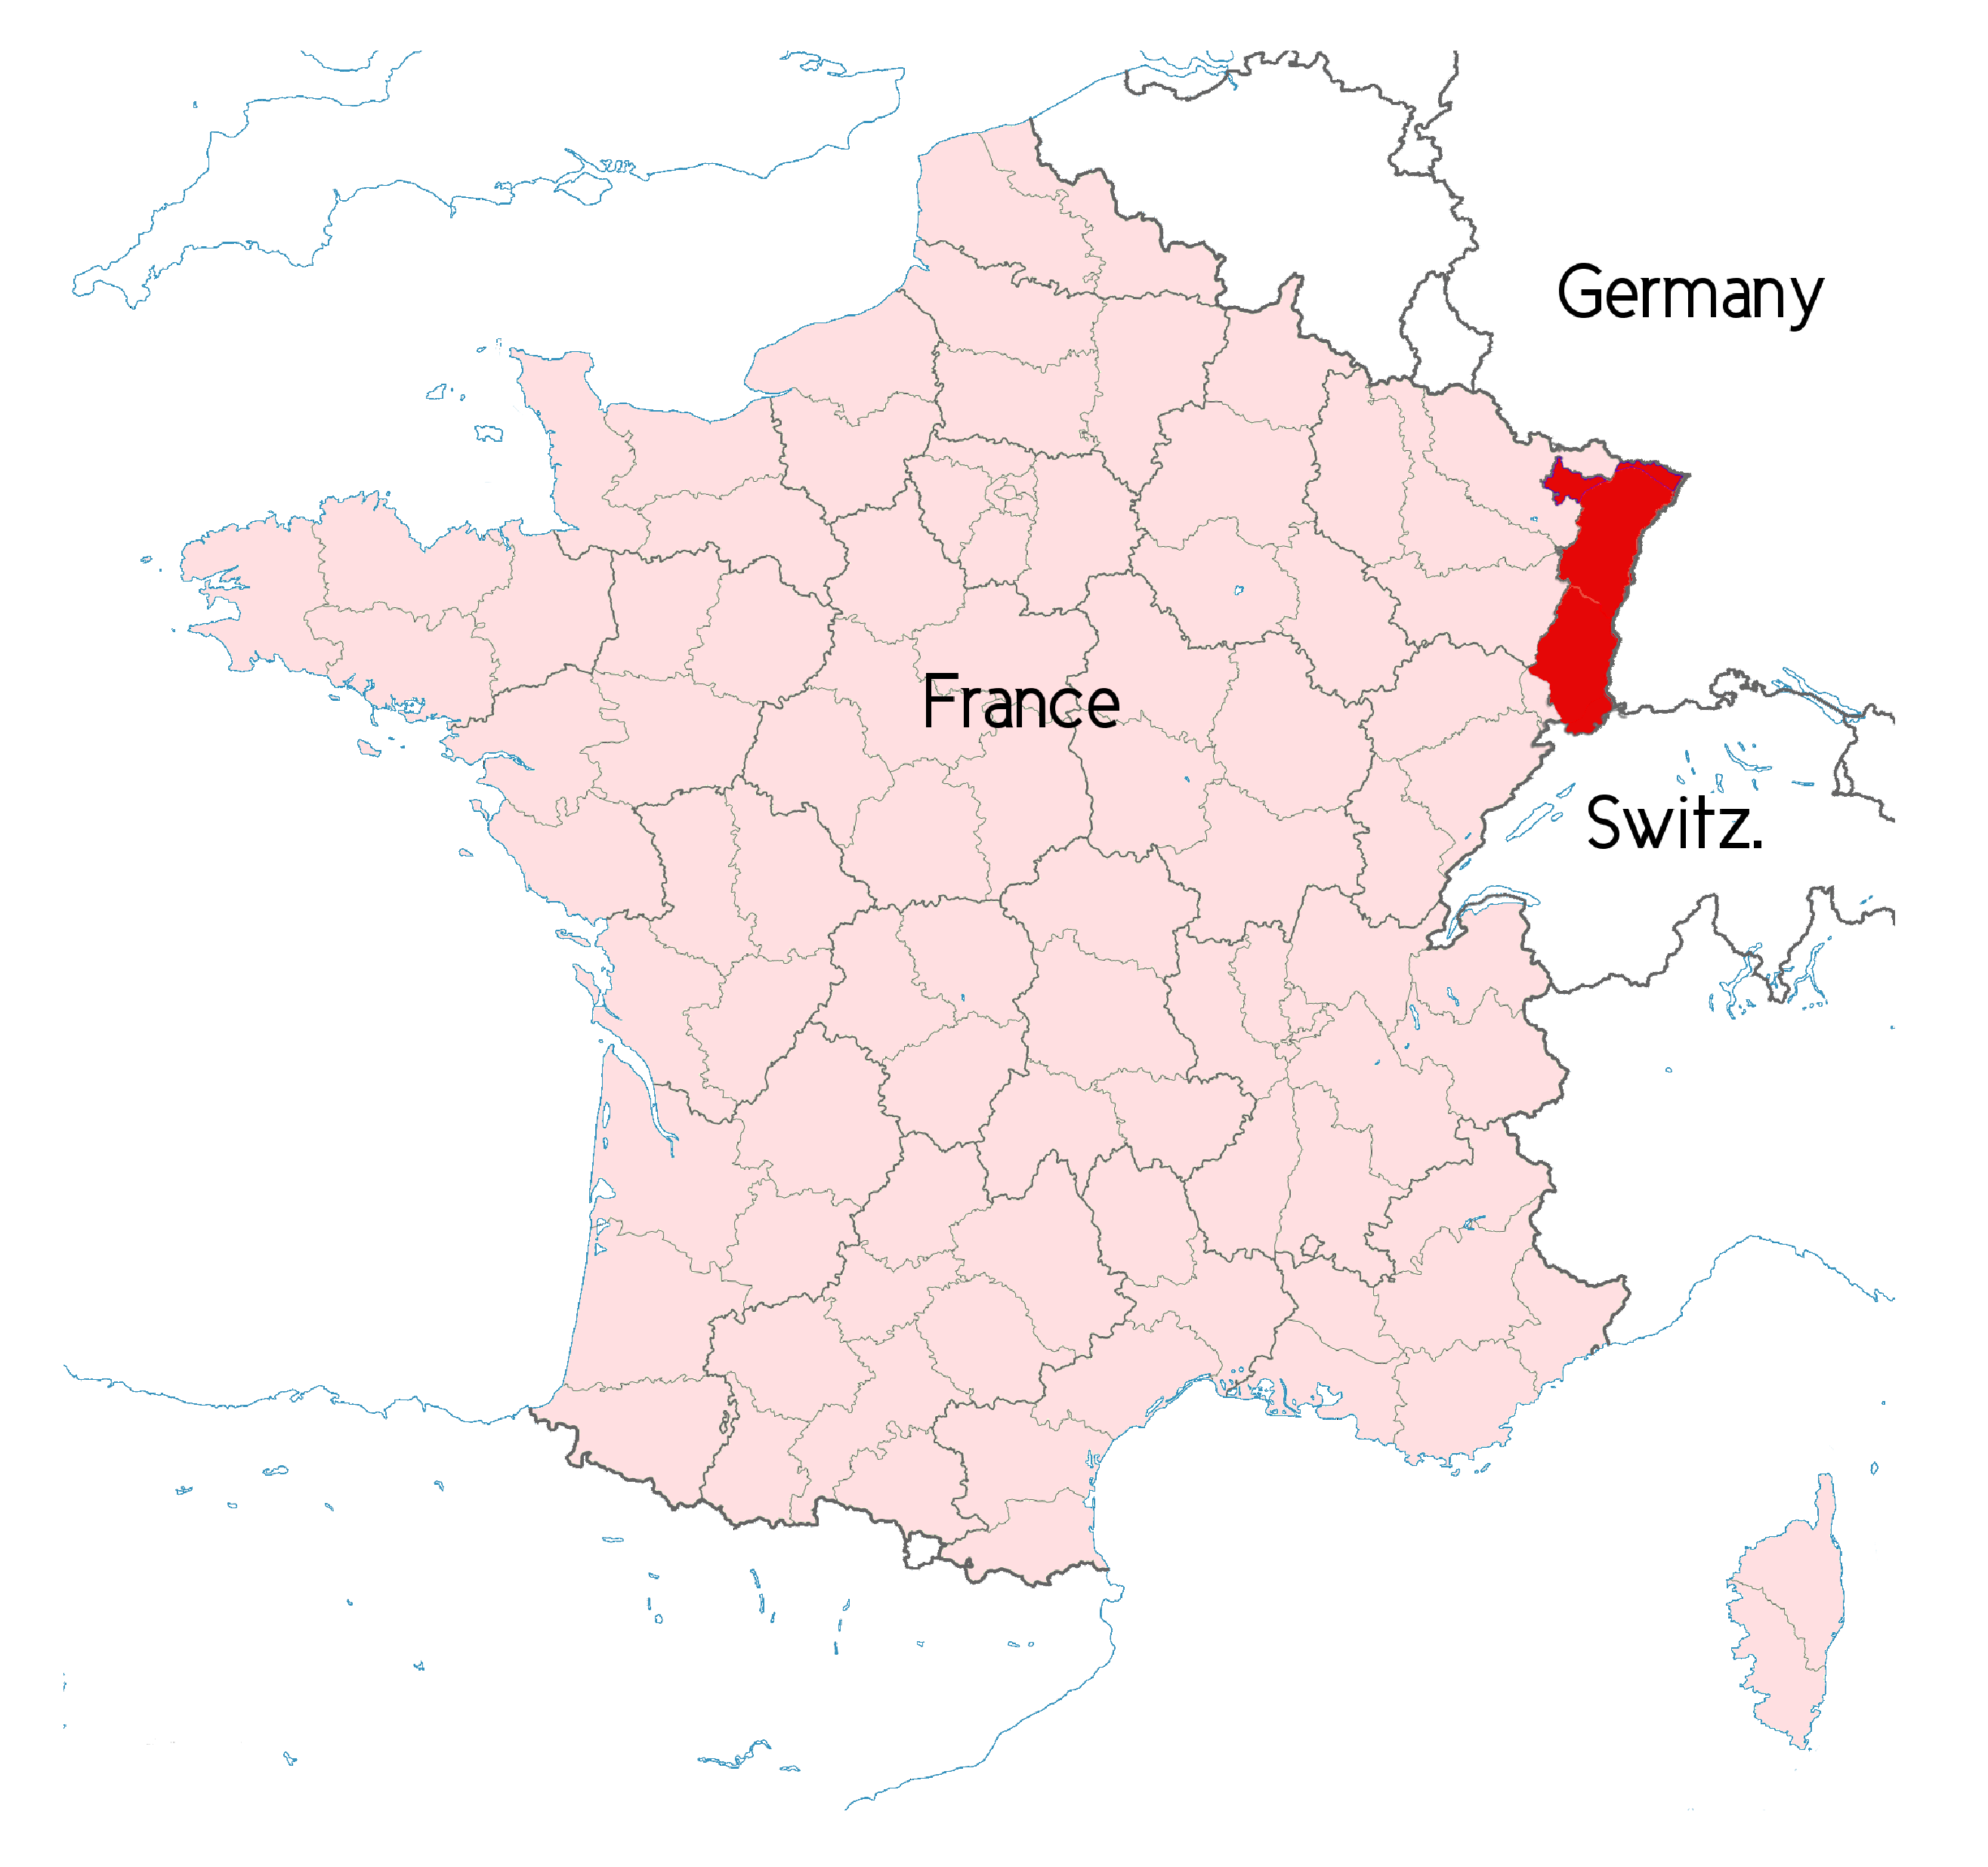
\includegraphics[width=1.1\textwidth]{figures/France-uni.png}};
        \end{tikzpicture}
      \end{column}
      \begin{column}{0.6\textwidth}
        \begin{itemize}
          %\visible<2->{
        \item Continuum de dialectes alémaniques.
        \item Pas de norme orthographique établie. 
        \item Population majoritairement bilingue.
        \item \textbf{550,000 locuteurs en 1999}\footnotemark[1].
          %}
        \end{itemize}
      \end{column}
    \end{columns}
    
    \visible<2->{\begin{center}
      \small
      %incompatible with footnote
      %{\setstretch{2.0}
      \vspace{-0.5cm}
      \textit{Mer Müess mache ass d'Kerisch mittess im dorf blieb.} \\~\\
      \scriptsize
      \vspace{-0.2cm}
      (Nous devons garder l'église au centre du village.) \\~\\
      %}
      
      \end{center}
      }
    \footnotetext[1]{Selon  \cite{institut_2004}.}
  }
\end{frame}

\subsection{Conditions of the experiment}
\begin{frame}{Conditions initiales}
  \Wider[4em]{
    \begin{alertblock}{L'alsacien, une langue peu dotée}
      \vspace{-0.1cm}
      \begin{itemize}
      \item Un lexique externe~\cite{bernhard_es_2013}.
      \item Un \textbf{corpus de référence minimal} (102 phrases).
      \visible<2->{\item Peu de ressources brutes libres de droit.}
      \end{itemize}  
    \end{alertblock}
    \vspace{-0.3cm}}
\begin{columns}
    \begin{column}{0.2\textwidth}
      \begin{tikzpicture}
        \node (img0) {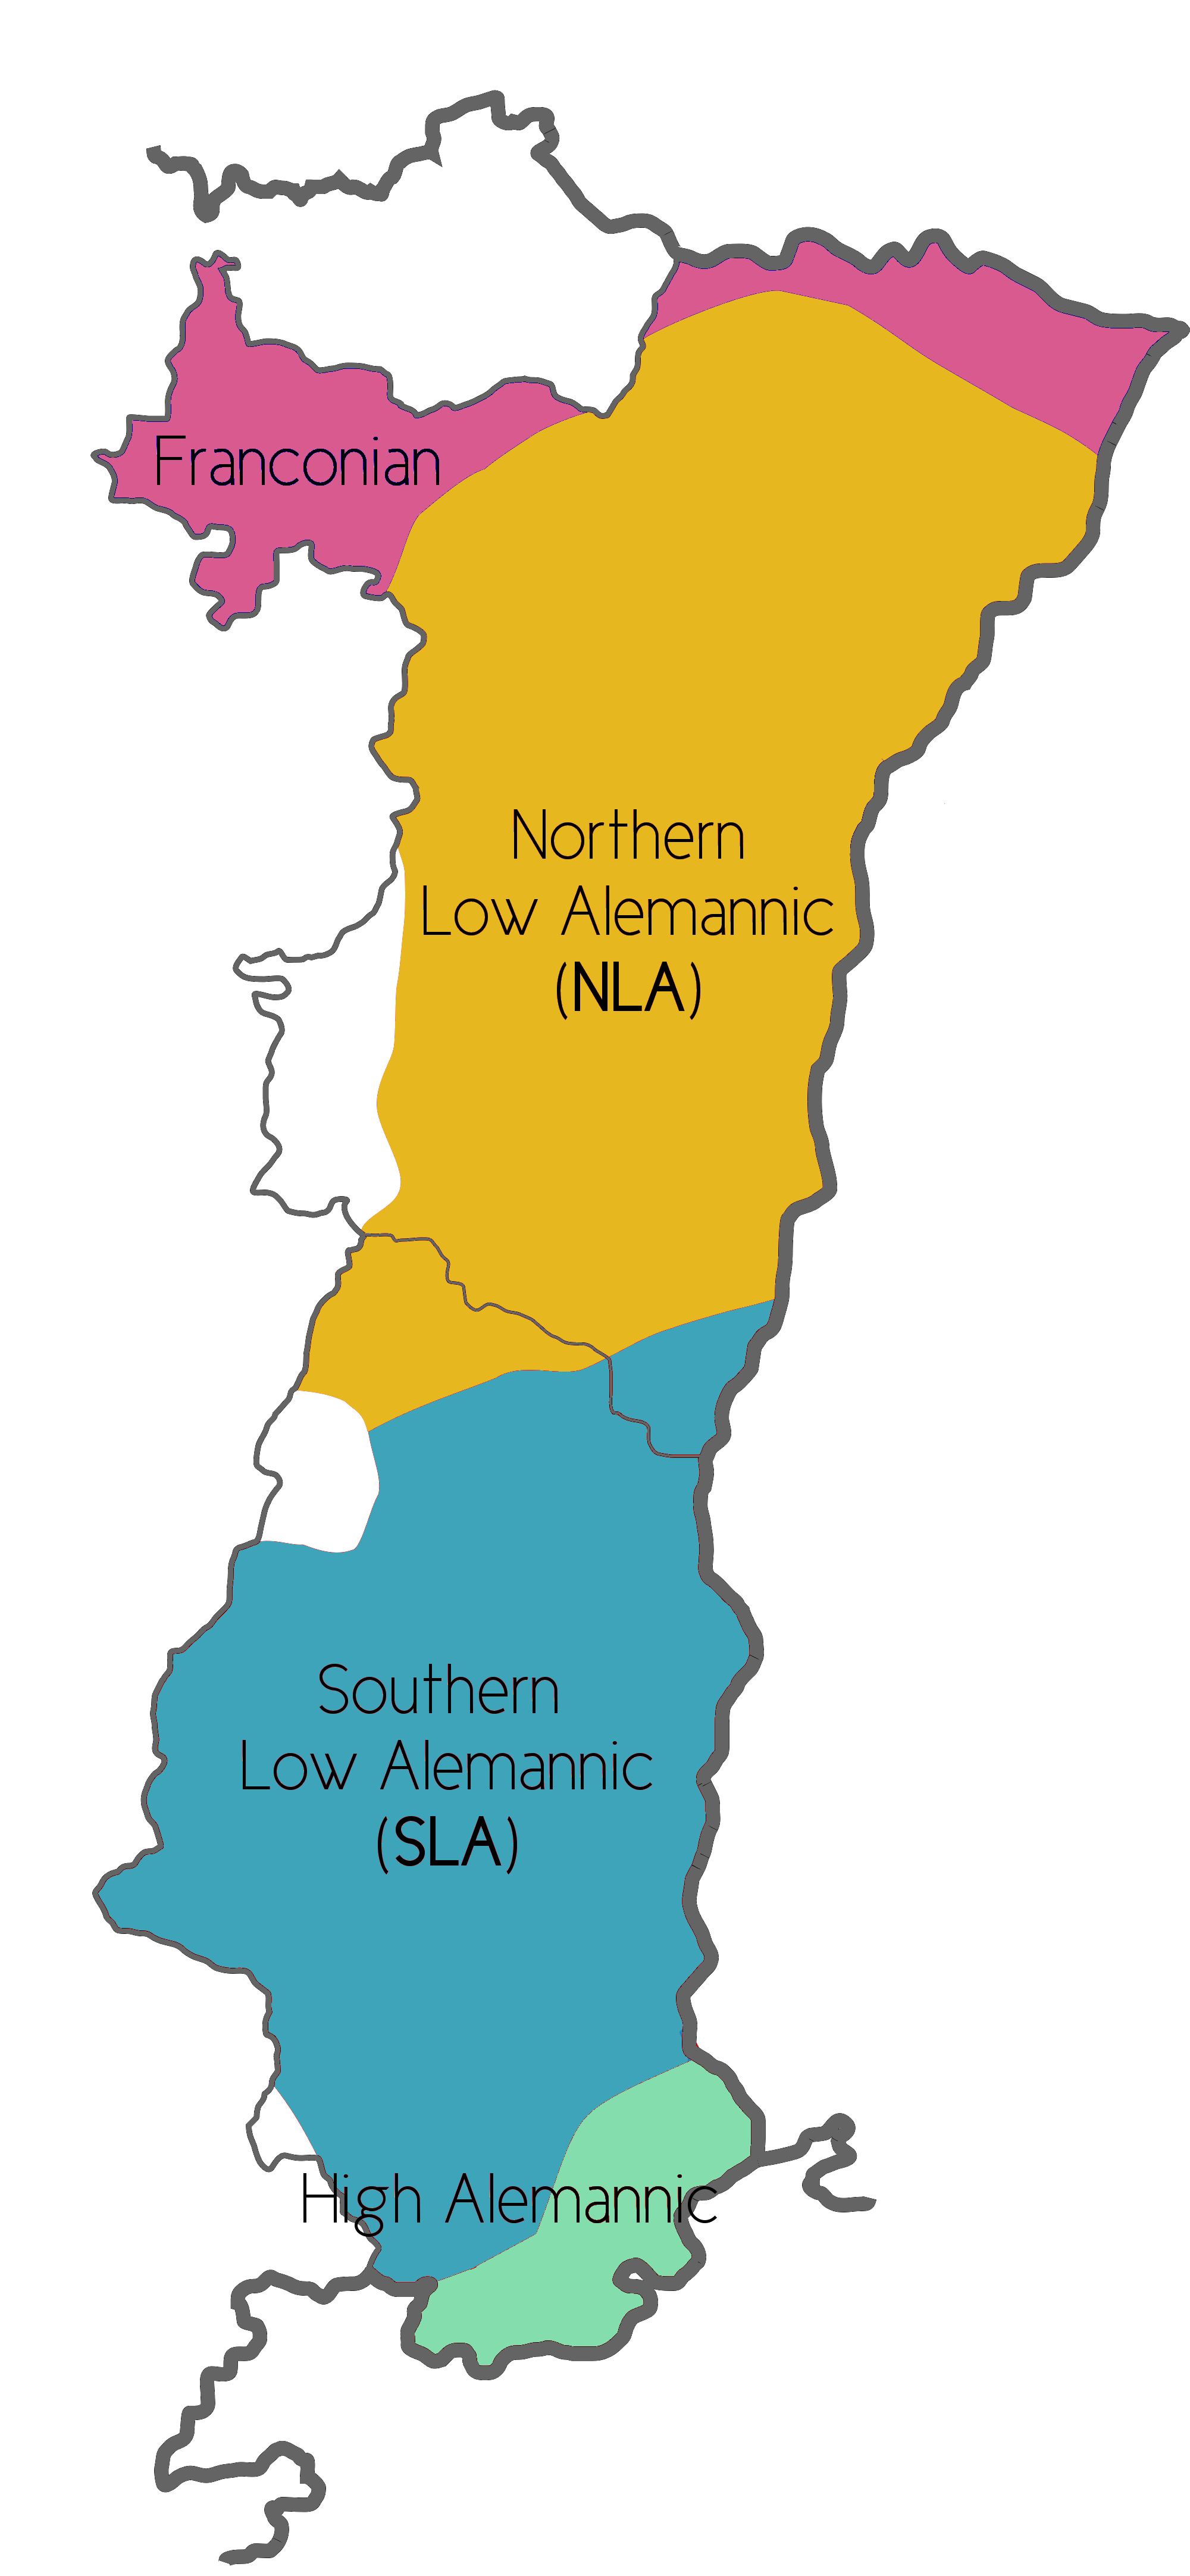
\includegraphics[height=5.5cm]{figures/Elsass.png}};
      \end{tikzpicture}
    \end{column}
    \begin{column}{0.8\textwidth}
      %\resizebox{\linewidth}{!}{
        \begin{table}[]
        \centering
        \small	
        \begin{tabular}{l|l|c|c}
          \toprule
          & Source & \multicolumn{2}{l}{Nb. tokens} \\ \hline
          \multicolumn{1}{l|}{\multirow{3}{*}{Corpus de référence}} & \multirow{2}{*} \nla\tool{Wikipédia} & {875} & \multirow{3}{*}{1.468} \\\cline{2-3} 
          \multicolumn{1}{l|}{} & \sla Recette de cuisine  & 362 &  \\ \cline{2-3} 
          \multicolumn{1}{l|}{} & \sla Pièce de théâtre
          & 231 & \pause \\ \hline \hline 
          \multicolumn{1}{l|}{Corpus Brut} & \nla \tool{Wikipédia}  & \multicolumn{2}{c}{8.833 (65\% annoté)} \\ \toprule  
        \end{tabular}
     %}
      \end{table}
    \end{column}
  \end{columns}
    
\end{frame}


\begin{frame}{Conditions initiales}
  \Wider[4em]{
    \begin{alertblock}{L'alsacien, une langue peu dotée}
      \vspace{-0.1cm}
      \begin{itemize}
      \item Un lexique externe~\cite{bernhard_es_2013}.
      \item Un \textbf{corpus de référence minimal} (102 phrases).
      \item Peu de ressources brutes libres de droit.
      \end{itemize}  
    \end{alertblock}
    \vspace{-0.3cm}
    \begin{alertblock}{Pas d'outil de TAL spécifique à l'alsacien}
    \end{alertblock}
    
    
    \vspace{-0.2cm}
    \hrulefill\par
    \vspace{-0.2cm}
    \visible<3->{\begin{exampleblock}{Outils d'annotation en partie du discours existant (POS taggers)}
        \vspace{-0.1cm}
        \begin{enumerate}
        \item German \tool{TreeTagger}~\cite{Schmid1997}\footnote{Utilisé selon la méthodologie décrite par \cite{bernhard_es_2013}}.
          \smash{\raisebox{1.8\dimexpr0.3\baselineskip-6.3\itemsep+5.5\parskip}{$\left.\rule{0pt}{1.5\dimexpr1\baselineskip+2\itemsep-1\parskip}\right\}$\ \parbox{2.8cm}{\center utilisés comme \\ \textbf{outils de pré-annotation}}}}  
        \item \tool{MElt}~\cite{Denis2010} \\ (78\% d'exactitude avec 50 phrases,\\ réentraîné régulièrement). 
        \end{enumerate}
    \end{exampleblock}}
    \vspace{-0.3cm}
    \visible<4->{
      \begin{exampleblock}{Une petite communauté de locuteurs actifs et connectés.}
        \small
        %\centering
        Groupes \tool{Facebook} dialectophones, Wikipédia alémanique (20.000 mots), pages personnelles etc.
      \end{exampleblock}
    }
  }
\end{frame}



\begin{frame}{Notre objectif}
  Faire annoter un corpus de l'alsacien en parties du discours
  \begin{center}
    \large
    grâce à une plateforme légèrement ludifée mettant à contribution des locuteurs motivés.
  \end{center}
\end{frame}


\section{\tool{Bisame}\thinspace - une plate-forme légèrement ludifiée}
\begin{frame}{Plan}
  \setbeamertemplate{section in toc}[sections numbered]
  \tableofcontents[currentsection,hideothersubsections]
\end{frame}

\subsection{Présentation de la plate-forme}
\begin{frame}{\tool{Bisame}}
  \Wider[4em]{
    \begin{tikzpicture}
      \node (img0) {\includegraphics[width=1\textwidth]{figures/frontpage.png}};
      \pause
      \node (img1) at (img0) {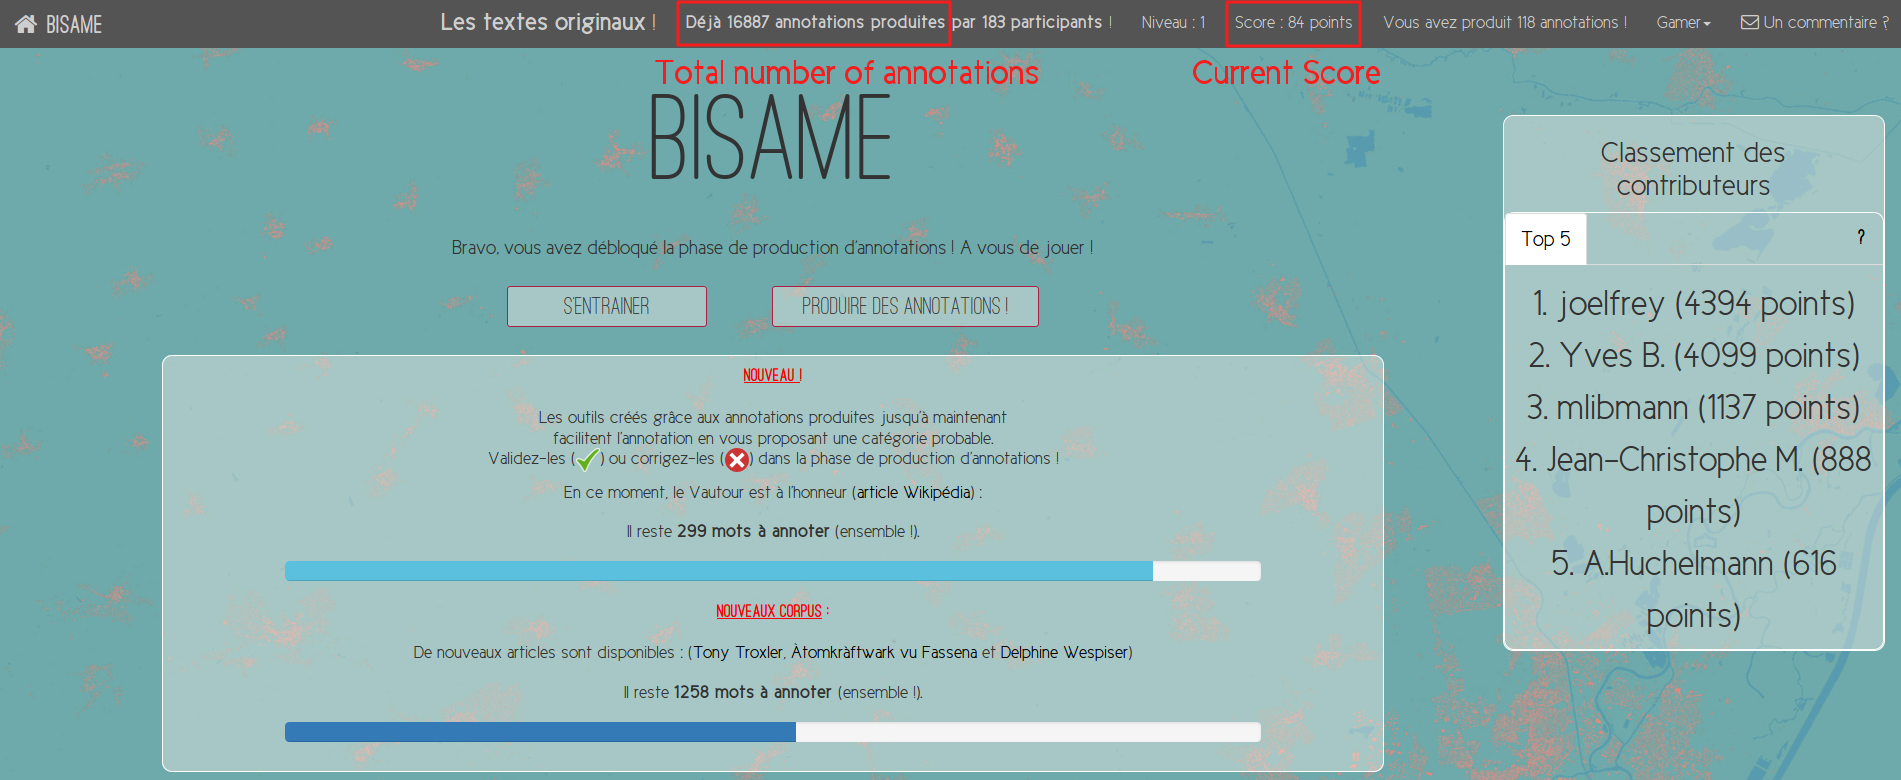
\includegraphics[width=1\textwidth]{figures/frontpage-1.png}};
      \pause
      \node (img2) at (img0) {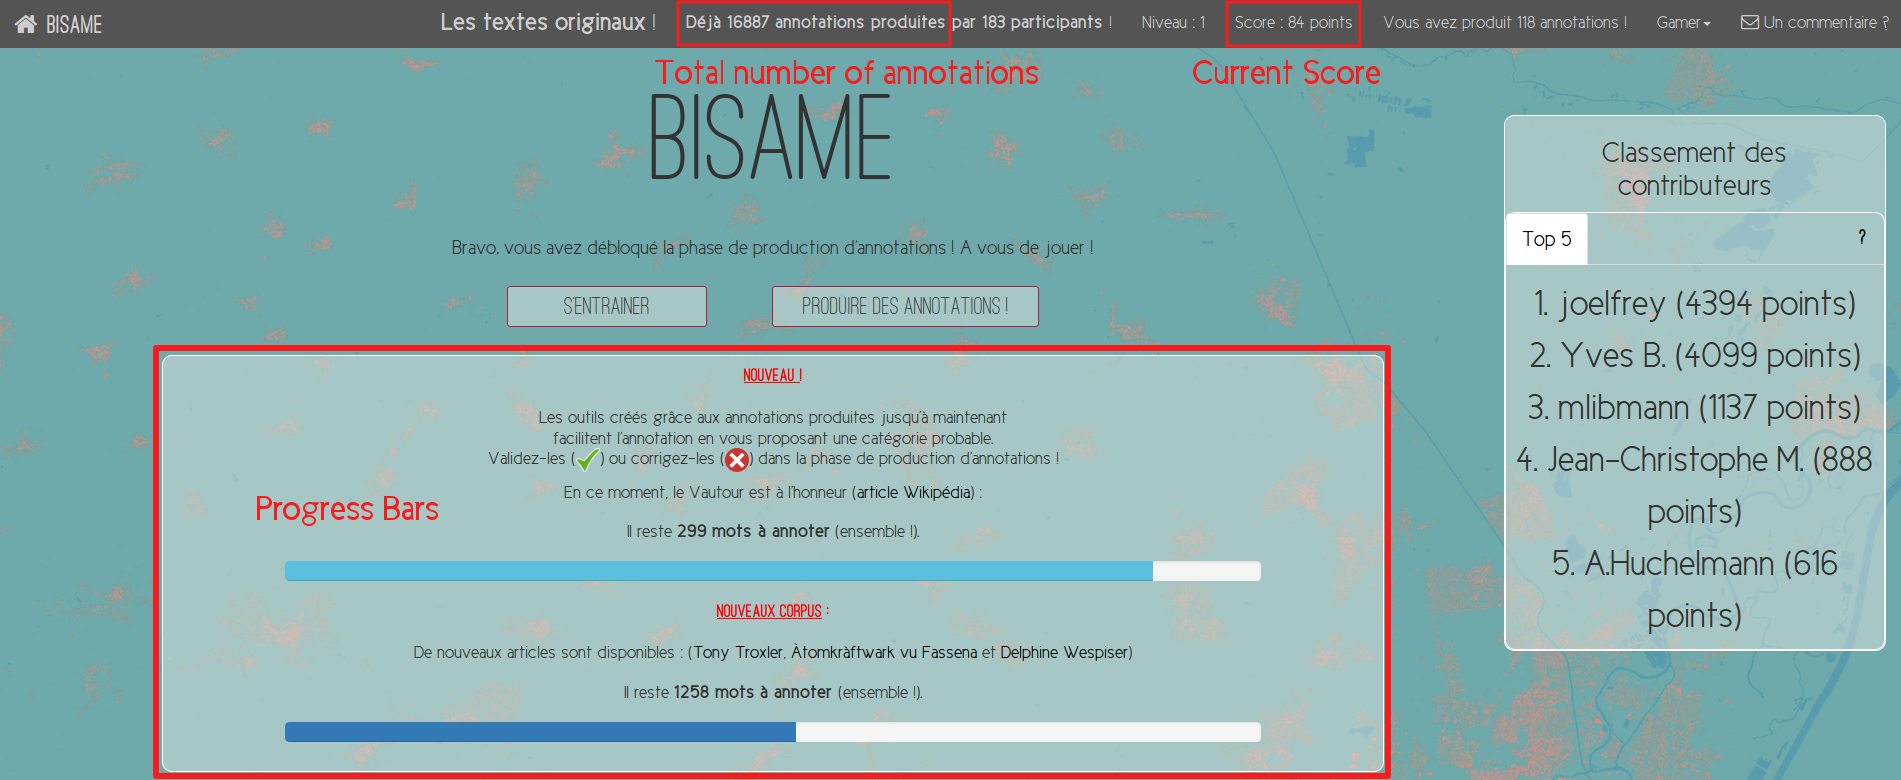
\includegraphics[width=1\textwidth]{figures/frontpage-2.png}};
      \pause
      \node (img3) at (img0) {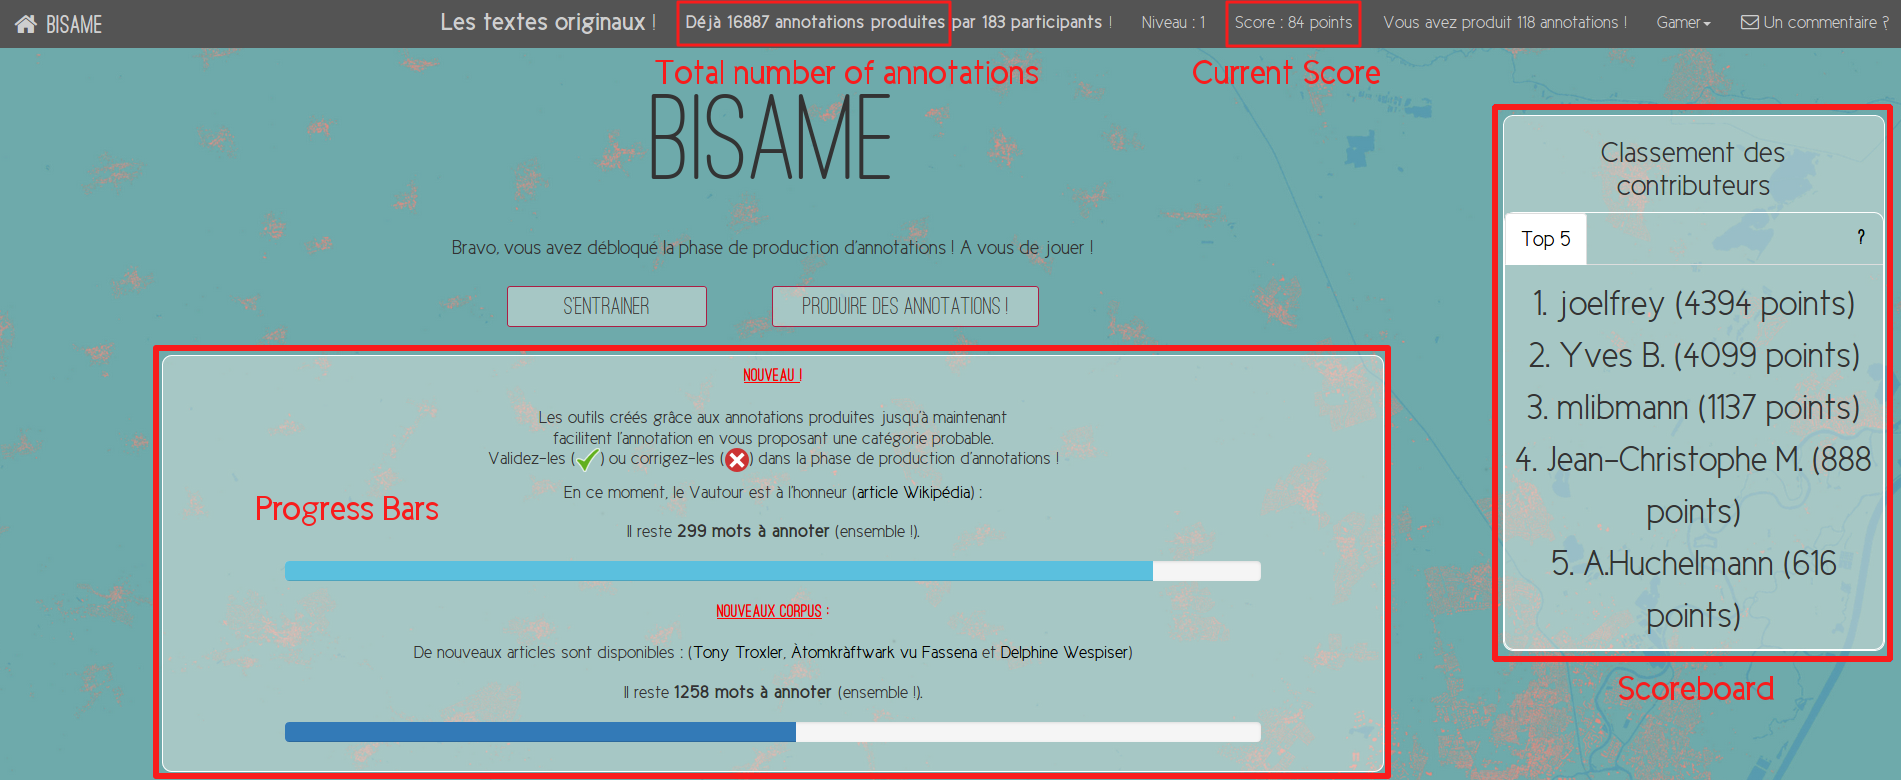
\includegraphics[width=1\textwidth]{figures/frontpage-3.png}};
    \end{tikzpicture}  
  }   
\end{frame}

\begin{frame}{L'annotation grâce à Bisame}
  En fonction des résultats de la pré-annotation :
  \begin{center}
    \visible<2->{Si \tool{Treetagger} \textcolor{red}{!=} \tool{MElt}: \\

    \begin{figure}
      
      \includegraphics[width=0.95\textwidth]{figures/annot2.png}

    \end{figure}}
    \visible<3->{Si \tool{Treetagger} \textcolor{green}{=} 	\tool{MElt}: \\
      \begin{figure}
        

        \includegraphics[width=0.95\textwidth]{figures/annot1.png}
      \end{figure}
    }

    
  \end{center}
\end{frame}
\subsection{Résultats}
\begin{frame}{Les résultats}
  \Wider[3em]{
    \begin{itemize}
    \item \textbf{42 participants} ont produit \textbf{8.833 annotations} sur le \uline{corpus brut}\footnotemark[1] \thinspace en 59 jours. \cite{Millour2017}.
    \item \textbf{F-mesure} moyenne de \tool{Bisame} sur le \uline{corpus de référence} : \textbf{92\%}.
    \end{itemize}
  }
  \metroset{block=fill}
  \visible<2->{
    \begin{exampleblock}{Produits de l'expérience}
      \pause
      \begin{itemize}
      \item Un nouveau \textbf{corpus annoté} de 5.725 tokens.
      \item<2-> L'\textbf{outil d'annotation} (\tool{MElt$_{ALS}$}~\cite{Denis2010}), fonctionnel pour l'alsacien avec \textbf{81\%} d'exactitude sur le sous-corpus de référence de la même variante dialectale.
      \end{itemize}    
    \end{exampleblock}
  }
  \visible<3->{
    \begin{table}[h!]
      \begin{tabular}{lcc}
        \toprule
        & \multicolumn{1}{l}{German \tool{TreeTagger}} & \multicolumn{1}{l}{\tool{MElt$_{ALS}$}} \\ \hline
        \sla Pièce de théâtre     & 83\%                                       & 66\%                     \\ \hline
        \nla Article Wikipédia & 85\%                                       & 84\%                   \\
        \toprule
      \end{tabular}
    \end{table}
  }
  \footnotetext[1]{16.628 annotations ont été effectuées au total.}
\end{frame}



\section{Analyse détaillée des résultats}
\begin{frame}{Plan}
  \setbeamertemplate{section in toc}[sections numbered]
  \tableofcontents[currentsection,hideothersubsections]
\end{frame}



\begin{frame}{La participation}
  \Wider[4em]{\begin{figure}[h!tbp]
      \begin{center} 
        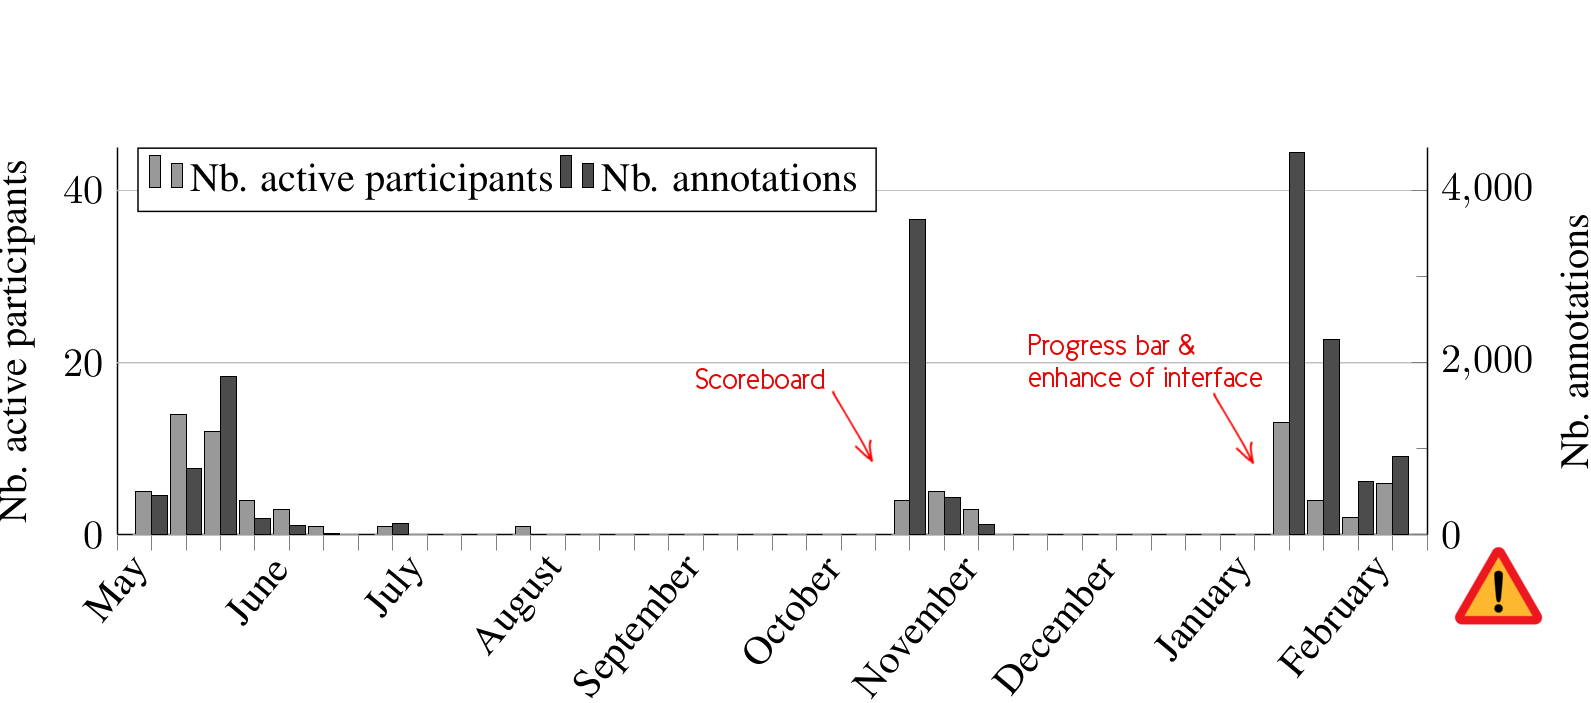
\includegraphics[width=1\textwidth]{figures/graphique-2.png}
      \end{center}
  \end{figure}}
  \\
  
  \bigskip
  \begin{columns}[]
    \begin{column}{0.30\textwidth}
      Mai 2016: \\
      
      \bigskip
      \visible<2->{Janvier 2017 : }
    \end{column} 
    \begin{column}{0.8\textwidth}
      29 participants ont produit 3.000 annotations. \\
      
      \bigskip
      \visible<2->{15 participants ont produit plus de 7.000 annotations.}

    \end{column}
  \end{columns}
  
\end{frame}

\begin{frame}{L'annotation sur le corpus de référence}

  
\end{frame}

\begin{frame}{Les performances de \tool{MElt$_{ALS}$}}

  
\end{frame}



\begin{frame}{Conclusion}
  \begin{itemize}
  \item General approach is promising but the platform is not attractive enough. \pause
  \item Basic features and language defense engagement are not sufficient to maintain \textbf{volition} (that confirms \cite{Munro2013}'s observations).  \pause
    %although it's hard to correlate precisely the progress observed across the experiment to the gamification features (given the low number of participation and there may have been combined effects) we still observed that the scoreboard indeed generated ephemeral competition between players.
%  \item Feedback from users: it's too hard or too boring.
  \item Gamification seems to help enhancing participation. 
  \end{itemize}
%  Figure out the right balance between easing the task, making it enjoyable and producing quality annotations in a lightweight platform. while taking care of not INTRODUCING a BIAS that could not be corrected !
\end{frame}

\begin{frame}{Conclusion}
  \begin{exampleblock}{\center Perspectives : \\}
    \begin{itemize}
    \item Reinforce community feeling \textit{within} the platform thanks to \textbf{social incentives}. %as they have been appreciated so far and have proved their efficiency elsewhere
    \item Work on autonomy (reminder e-mails, ``one sentence per day'' system).
    \item Enable participants to \textbf{submit personal texts} \cite{Liberm2016}. 
    \item<2-> Adapt the platform to another language (Guadeloupean Creole).
    \item<2-> Try to manage better dialectal diversity in the written form. % and I take advantage of this talk to say that if you have some references on the subject I would me really glad to have them ! 
    \end{itemize}
  \end{exampleblock}
\end{frame}

\begin{frame}[standout]
  \textit{Merci vielmols!} \\~\\
  \scriptsize   	
  Merci !
  \begin{center}
    %{\setstretch{1.5}
    \normalsize
    \tool{Bisame}: \url{http://bisame.herokuapp.com} \\ 
    
    \includegraphics[width=0.02\textwidth]{figures/github-white.png}\enspace Github:         \url{https://github.com/alicemillour/Bisame}
    %}
  \end{center}
\end{frame}

%\appendix

%\begin{frame}[fragile]{Backup slides}
%  Sometimes, it is useful to add slides at the end of your presentation to
%  refer to during audience questions.
%
%  The best way to do this is to include the \verb|appendixnumberbeamer|
%  package in your preamble and call \verb|\appendix| before your backup slides.
%
%  \themename will automatically turn off slide numbering and progress bars for
%  slides in the appendix.
%\end{frame}

\begin{frame}[allowframebreaks]{References}

  \bibliographystyle{apalike}
  \bibliography{pres_atelier_corpus}
\end{frame}


\end{document}
